\section{Eulersche Phi-Funktion}

Die Eulersche Phi-Funktion, auch bekannt als eulersche Totientfunktion, ist eine von Leonhard Euler 1763 formulierte Funktion der Zahlentheorie, welche die Summe der teilerfremden Zahlen zu $n$ darstellt\cite{pacific}:

\begin{equation}
  \begin{aligned}
    &n \in \mathbb{N}^+\\
    &\left\{\,\varphi(n) \in \mathbb{N}^+\mid 0 \le \varphi(n) \le n-1 \right\}\\
    &\varphi(n) = n \times \prod_{p\mid{}n}\left(1-\frac{1}{p}\right)
  \end{aligned}
\end{equation}

$\varphi(n)$ ist der Totient von $n$.

\begin{align}
  \varphi(5)&= 4 && \text{$\varphi(5) = n-1$, da n prim ist}\label{totative:1}\\
  \varphi(9)&= 6 && \text{teilerfremd zu $1_1$, $2_2$, $4_3$, $5_4$, $7_5$, $8_6$}\\
  \varphi(8)&= 4 && \text{teilerfremd zu $1_1$, $3_2$, $5_3$, $7_4$}\label{totative:2}\\ 
  \varphi(16)&= 8 && \text{teilerfremd zu $1_1$, $3_2$, $5_3$, $7_4$, $9_5$, $11_6$, $13_7$, $15_8$}\label{totative:3}
\end{align}

In Gleichungen \eqref{totative:1}, \eqref{totative:2} und \eqref{totative:3} sind zwei Spezialfälle für Werte $n$ der eulerschen Phi-Funktion zu sehen; Primzahlen und Potenzen zur Basis zwei:

\begin{enumerate}
  \item Für $n \in \mathbb{P}$ ist $\varphi(n)$ immer gleich $n-1$.\cite{mw02}
  \item Für $n=2^k \land k \ge 1$ ist $\varphi(2^k)=2^{k-1}$.
\end{enumerate}

Weitere Attribute der Funktion und ihrer Parameter sind:

\begin{enumerate}
  \item Für $n \ge 3$ ist $\varphi(n)$ immer  gerade, sprich $\varphi(n)=2k$.\cite{mw02}
  \item Konventionell ist $\varphi(0)=1$ definiert.\cite{mw02}
\end{enumerate}

Die eulersche Phi-Funktion findet auch Anwendung in einer Verallgemeinerung des kleinen fermatschen Satzes, welche von Euler auch 1763 publiziert wurde:

\begin{equation}
  a^{\varphi(n)} \equiv 1\pmod(n)
\end{equation}

Für alle Zahlen $a$ welche teilerfremd zu $n$ sind.\cite{mw03}

\ref{totative_dist} zeigt die Verteilung von $\varphi(n)$ für die ersten eintausend Werte $n$.

\begin{figure}[H]
  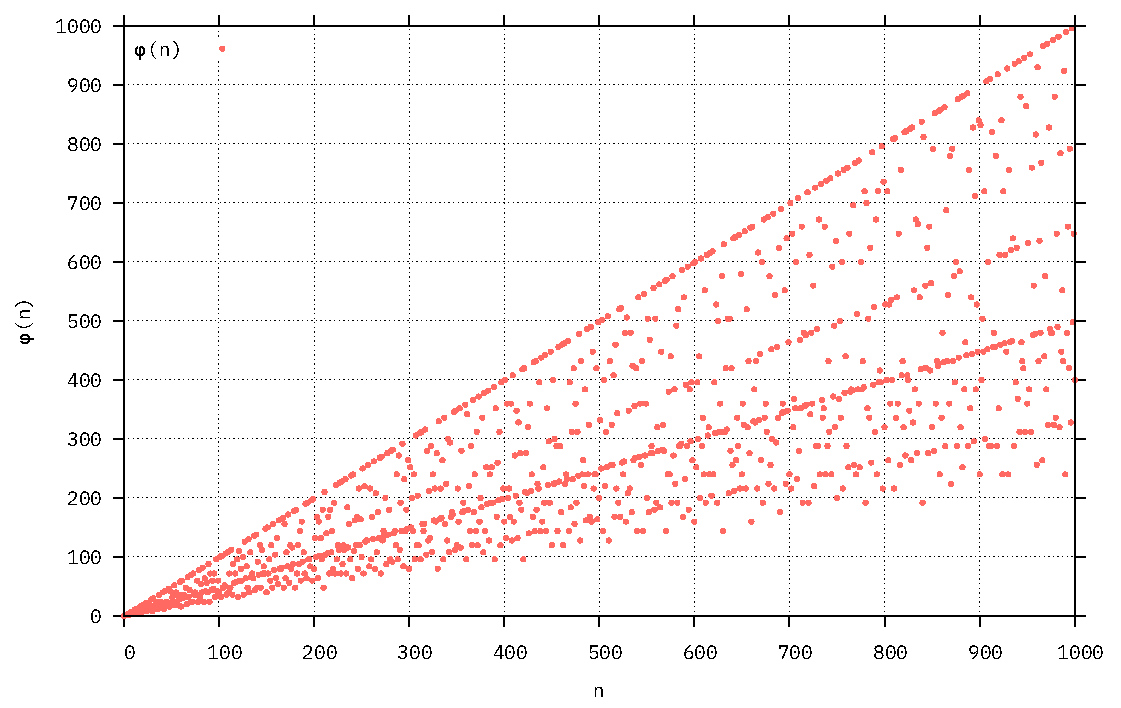
\includegraphics{totient.pdf}
  \caption{Eulersche Phi-Funktion $\varphi(n)$ für $\left\{\,n \in \mathbb{N}\mid 0 \le n \le 1000 \, \right\}$}
  \label{totative_dist}
\end{figure}
